\documentclass[a4paper, 12pt]{report}
\usepackage[pdftex]{graphicx}
\usepackage[autostyle]{csquotes}
\usepackage[backend=bibtex,style=numeric,sorting=none]{biblatex}
\usepackage{caption}
\usepackage{subcaption} % for subfigure
\usepackage{hyperref}
\usepackage{amssymb}
\usepackage{tabularx}
\usepackage{multicol}
\usepackage{algpseudocode}
\usepackage{amsthm} % for theorem
\usepackage{algorithm}
\addbibresource{bibliography}

\theoremstyle{plain}
\newtheorem{thm}{Theorem}[chapter] % reset theorem numbering for each chapter

\theoremstyle{definition}
\newtheorem{defn}[thm]{Definition} % definition numbers are dependent on theorem numbers
\newtheorem{exmp}[thm]{Example} % same for example numbers

\begin{document}
\pagenumbering{roman}
\begin{titlepage}
\begin{center}

{\Huge \bfseries
Optimizing Join Enumeration \\
in Transformation-based Query Optimizers\\
}~\\[1cm]

% The '~' is needed because \\ only works if a paragraph has started.

{\large \bfseries
B.Tech. Project 1st Stage Report
}~\\[0.40cm]

{
Submitted in partial fulfilment of the requirements for the degree of
}~\\[0.20cm]

{\large \bfseries
Bachelor of Technology (Honors)
}\\[2.75cm]
\end{center}

\begin{multicols}{2}
\begin{flushleft}
{\large
\textit{Student:} \\
\textbf{Anil Shanbhag} \\
\textbf{Roll No: 100050082}
}
\end{flushleft}
\columnbreak
\begin{flushright}
{\large
\textit{Guide:} \\
\textbf{Dr. S. Sudarshan}
}
\end{flushright}
\end{multicols}

\vfill

\begin{center}

\includegraphics[width=4cm]{Figures/iitbblack.jpg}~\\[1cm]

{\large
Department of Computer Science and Engineering\\
Indian Institute of Technology Bombay\\
Mumbai 400076, India\\
}

\end{center}
\end{titlepage}
\chapter*{}
\begin{center}
\textbf{Abstract}
\end{center}
Transformation-based query optimizers explore the search space exhaustively using transformation rules. This report looks at a specific problem of enumeration of all valid bushy join trees without cross products. We show that existing rule sets either fail to explore the complete space or explore the entire space but generate exponential number of duplicates. A literature survey of  techniques used for join enumeration in different settings is presented including DP-based and memoization-based algorithms for plan generation. We present two new methods for enumerating the search space which perform superior to existing methods.
\addcontentsline{toc}{chapter}{Abstract}
\begin{center}
{\large \bfseries
Acknowledgement
}~\\[1cm]
\end{center}
\begin{flushleft}
{
I wish to express my sincere gratitude and indebtedness to my guide, \\ Dr. S. Sudarshan for his constant support and guidance	 throughout the project. 
}~\\[1.5cm]
{
Anil Shanbhag\\
B.Tech. IV\\
CSE, IIT Bombay
}
\end{flushleft}

\tableofcontents
\pagenumbering{arabic}
\chapter{Introduction}

For a DBMS that provides support for a declarative query
language like SQL, the query optimizer is a crucial piece of software. The declarative nature of a query allows it to be translated into many equivalent evaluation plans. The process of choosing a suitable plan from all alternatives is known as query optimization. The basis of this choice are a cost model and statistics over the data. Essential for the costs of a plan is the execution order of join operations in its operator tree, since the runtime of plans with different join orders can vary by several orders of magnitude. 

\section{Transformation-based Query Optimizers}
Long ago, Ono and Lohman\cite{ono1990measuring} gave a lower bound of $O(3^n)$ with n the number of relations, on the complexity join enumeration, by counting how many join operators are considered in the bottom-up dynamic programming enumeration algorithm of System R and Starburst. Bottom-up dynamic programming and top-down memoization based join enumeration algorithms have been found which achieve this lower bound and hence are very efficient for join enumeration. However there is advantage to reordering other operators and choosing among the new alternatives based on cost estimation. DP based techniques have been extended to deal with other operators (eg: aggregations, outer joins), however there is no general technique for extension. For example, to deal with with sub-queries Seshadri et al suggested a clever iterative algorithm in which an extended bottom-up enumeration module is called many times - but we are forced beyond bottom-up framework. \\

Rule-based query optimizers are extensible as they are described using a set of transformation rules. All possible rules are applied on each alternative until no new information is produced. However the trade-off of rule-based optimizers is efficiency.

\section{The Search Space}
An exhaustive search for an optimal solution over all possible operator trees is computationally expensive. To decrease complexity, the search space must be restricted. For the optimization problem discussed in this report, a well-accepted heuristic is applied: We consider all possible bushy join trees, but exclude cross products from the search, presuming that all considered queries span a connected query graph \cite{ono1990measuring}. Our goals are:
\begin{itemize}
	\item Complete space enumeration
	\item Remain in the space of cross product free join trees
	\item Avoid generation of duplicates
\end{itemize}

The goal is to enable cost-based selection of alternatives that are generated via transformation rules, while being as efficient as top-down join enumerator.
 
\section{Organization of the Report}
The rest of the report is organized as follows:
In Chapter 2, we introduce general concepts in traditional query optimization. In Chapter 3, a literature survey of different join enumeration algorithms is presented. In Chapter 4, we prove the in-effectiveness of existing rule sets. In Chapter 5, we present a new rule set which improves on the drawbacks of existing rule sets. In Chapter 6, we present a new method for join enumeration in a rule-based setting. In Chapter 7, we look into possible future steps in this direction. Finally we conclude the report in Chapter 8.  
\chapter{Query Optimization Overview}

In this chapter, we describe the design of cost-based transformational query optimizer, based on Volcano Framework. \\

Query optimization is probably the most critical component of modern database systems, since the ubiquity of the database system depends on the efficiency with which a user's queries are executed by the system. As queries submitted to the database system by the user using a high-level declarative language do not specify an execution plan, it is the job of the optimizer
to generate a good plan, and query optimization can achieve substantial improvements in runtime and resource usage during execution of the query. \\

Traditionally, query optimizers follow a three step approach \cite{roy2000efficient}:
\begin{itemize}
	\item  Generate all execution plans that are logically equivalent to the user-submitted query.
	\item Estimate the cost of executing each of the alternate plans.
	\item Search through the space of all generated plans to find the plan with least cost.
\end{itemize}

\section{Space of Logically Equivalent Plans}
All plans that compute the same result, having the same properties, as that computed by the original query plan, are called to be logically equivalent to the given query. \\

The parser parses the query to generate a query tree. From the initial query tree, the space of all logically equivalent plans can be generated using transformation rules.

\subsection{Logical Plan Space}
The initial query tree consists of logical operators which are like the relational operators select, project, join, etc, and which do not specify the physical algorithm to be used during actual computation. All logical plans that are equivalent to the initial query plan constitute the logical plan space of the query. \\

The logical plan space can be generated by applying logical transformation rules to operators in the logical plan of the query. The new plans generated are further transformed whenever possible, until no new plans can be generated using the given set of rules.

\subsection{Physical Plan Space}
The logical plan must be converted to a physical plan than can be executed on the database system. The implementation rules define which logical operator may be implemented using which physical algorithm. \\

The physical plan space is generated by applying the implementation rules to all plans in the logical plan space.

\section{Logical Space Generation}
We describe the generation of logical plan space in greater detail. The logical plan space is the set of all semantically equivalent logical plans of the input query.

\begin{defn} 
A Logical Query DAG is a directed acyclic graph whose nodes can be divided into equivalence nodes and operation nodes; the equivalence nodes have only operation nodes as children and operation nodes have only equivalence nodes as children. 
\end{defn}

Given a set of rules, we construct a Logical Query DAG from the given input query and expand the DAG to encompass the space of all equivalent logical plans. For example, the query tree of Figure \ref{fig:joinabc}(a) for the query $(A \bowtie B \bowtie C)$ is initially represented in the LQDAG formulation, as shown in Figure \ref{fig:joinabc}(b). The equivalence nodes are shown as boxes, while the operation nodes are shown as circles. \\

The initial LQDAG is then expanded by applying all possible transformations on every node of the initial LQDAG representing the given query. In the example, suppose the only transformations possible are join associativity and commutativity. Then the plans $(A \bowtie (B \bowtie C))$ and $((A \bowtie C) \bowtie B)$, as well as several plans equivalent to these modulo commutativity can be obtained by transformations on the initial LQDAG of Figure \ref{fig:joinabc}(b). These are represented in the LQDAG shown in Figure \ref{fig:joinabc}(c). For exact algorithm refer to pseudocode of procedure \textsc{ExpandDAG} presented in Figure \ref{fig:expandDAG}.

\begin{figure}[here]
\begin{center}
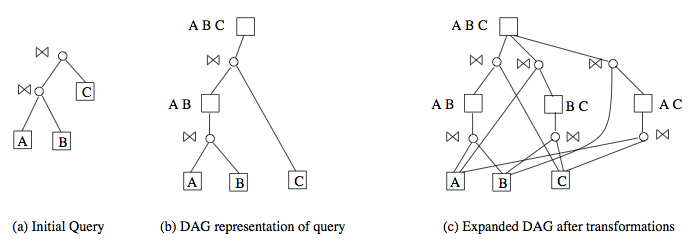
\includegraphics[width=14cm]{Figures/example_logical.png}
\end{center}
\caption{Logical Plan Space Generation for $A \bowtie B\bowtie C$}
\label{fig:joinabc}
\end{figure}

\begin{figure}[here]
\begin{center}
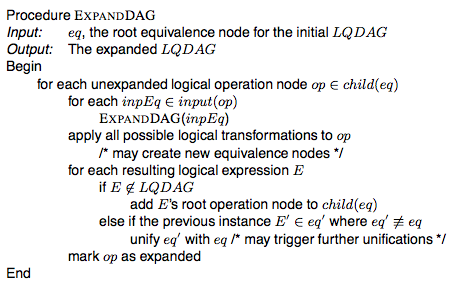
\includegraphics[width=11cm]{Figures/expandDAG.png}
\end{center}
\caption{Algorithm for LQDAG Generation}
\label{fig:expandDAG}
\end{figure}

\section{Cost Model}
The cost of executing a particular physical plan must be estimated for the purpose of finding the optimal plan. As the actual cost is not available during optimization, it is imperative for the estimates to be close to the actual costs in order to find the best plan. \\

The cost model defines how a cost is to be estimated for a particular operator when executed on the database. The optimizer makes use of database statistics, like histograms, and various other rules, for estimating the cost.

\section{Search for Optimal Plan}
The search strategy forms an important part of the optimization scheme. As there are exponentially many alternative plans to be considered, it is infeasible to enumerate all the plans and pick the one with the lowest cost. The optimizer must incorporate pruning techniques to reduce the size of the search space that will be explored during optimization.

\chapter{Related Work}
In this chapter we describe prior work in the area of finding optimal join order.

\section{TreeOpt Algorithm}
Some of the earliest work on finding optimal join order was done by Ibraraki and Kameda\cite{ibaraki1984optimal}.  They describes an algorithm for finding the optimal nesting order for tree queries ie: queries whose join graphs form a tree for nested loop join. Finding a solution for general graphs is NP-Hard, however for this special case it is possible to find the optimal solution in polynomial time. \\

A cost function f is said to satisfy the \textit{adjacent sequence interchange} property (ASI property in short) if there exists a rank function $r_{f}$ such that $f(AS_{1}S_{2}B) <= f(AS_{1}S_{2}B)$ if and only if $r_{f}(S_{1}) <= r_{f}(S_{2})$. It is known that if a cost function $f$ satisfies the ASI property, an optimal sequence can be found in $O(n log(n))$ where the order constraints are series parallel. In our case, the order constraints are directed tree which is a special case of series parallel constraints. \\

Refer to Algorithm \ref{alg:treeopt}. Set one of the nodes in tree as root R, call \textsc{TreeOpt} $(T,R)$. Every node in the tree has a rank given by rank function $r_{f}$. Until we reduce the tree to a chain, find a wedge in the tree and reduce it a chain where the nodes are listed in the order of their rank. However there might be ordering constraints within in a chain. The subroutine \textsc{Normalize} in called on each chain prior to reduction which combines nodes $S_{i}$ and $S{j}$ in the chain if $r_{f}(S_{i}) > r_{f}(S_{j})$ and $S_{i}$ occurs before $S_{j}$, a new label $S_{k}$ is assigned for combined entity containing $S_{i} \cup S_{j}$ and its rank is recalculated.  \\

\textsc{TreeOpt} is called n times, each time with different node as root. In the end we have an optimal tree for each node as root. The tree with the lowest cost among these is  indeed the optimal tree. Complexity : $O(n^2 log(n))$.

\begin{algorithm}
  \caption{Finding Optimal Nesting Order for Tree Queries
    \label{alg:treeopt}}
	\begin{algorithmic}[1]
	\Function{TreeOpt}{$T,R$}
		\State $rt \gets$ directed tree rooted at R   
		\While {$rt$ is not a chain}
			\State Find a wedge in the tree $rt$
			\State Apply \textsc{Normalize} to each chain of the wedge.
			\State Merge the two chains into one by ordering the nodes by their ranks.		
		\EndWhile
	\EndFunction
  \end{algorithmic}
\end{algorithm}

For optimizing cyclic join graphs the strategy is to first transform the graph into an acyclic join graph before running \textsc{TreeOpt}. This acyclic join graph needs to chosen with care. Note that when ordering the nodes, the goal was to reduce the number of page fetches. This in nested loop join means keeping size of intermediary relation low. Hence one good candidate for the tree is Minimum Spanning Tree with edge weights as $|R_{i}||R_{j}| \sigma_{R_{i}R_{j}}$. However it is shown experimentally that this method is not reliable.

\section{Heuristic for Cyclic Queries}
\textsc{TreeOpt} generates optimal plan for any acyclic join graph in polynomial time. However for cyclic queries, it does a bad job at even producing a near optimal plan. Raghavan et al. \cite{raghavan2009multi} propose a new algorithm called FAB (Forward and Backward) algorithm for producing better plans for cyclic join graph in polynomial time. \\

FAB approach uses a global-impact based ordering, in which the global impact of each relation explored and used to decide the ordering. The global impact of a  relation $R_{i}$ is the product of the size of all other relations and join selectivity not related to $R_{i}$. Intuitively if node $R_{i}$ has least impact, it means that it itself has a combination of large size and low join selectivity. The FAB algorithm picks the node with least impact and puts it as the last node to be joined. It then recalculates the impact of each node after removing the element from the join graph. \\

This approach works quite well for cyclic join graphs but note it not guaranteed to produce optimal plan always. The paper proposes a query aware approach where given a query, we try to infer if the join graph is linear, acyclic or cyclic. For the first two, use the TreeOpt algorithm and for third use FAB. \\

Note that FAB and TreeOpt are both used to generate left deep join trees. They do not help in any way to find the optimal solution in the space of all bushy join trees. 

\section{DP and Memoization based join enumeration}
Two approaches have done well at exploring and finding the optimal plan in the space of all bushy join orderings : bottom-up join enumeration via dynamic programming and top-down join enumeration via memoization. Moerkotte and Neumann \cite{moerkotte2006analysis} presented an efficient dynamic programming based algorithm (\textsc{DPccp}). DeHaan and Tompa \cite{dehaan2007optimal} proposed an efficient top-down algorithm (\textsc{TDMinCutLazy}). Fender and Moerkotte \cite{fender2011new} proposed an alternative top-down join enumeration strategy (\textsc{TDMinCutBranch}), which is almost as efficient as \textsc{DPccp}. In the following year, Fender et al.\cite{fender2012effective} proposed another top-down enumeration strategy \textsc{TDMinCutConservative} which is currently the best.

\subsection{Generic Top-Down Enumeration}
Top-Down join enumeration has a clear advantage over Bottom-Up style as it enables pruning. We describe a generic top-down enumeration via \textsc{TDPlanGen} (see pseudocode in Figure \ref{fig:tdplangen}). Like in dynamic programming, TDPlanGen initializes the building blocks for atomic relations first (line 2). In line 3, the subroutine \textsc{TDPGSub} is called, which traverses recursively through the search space. At each invocation of \textsc{TDPGSub}, a connected subgraph $G_{|S}$ is given. If the best tree for this graph is not known, a suitable partitioning strategy is used to partition $S$ into two sets $S_{1}$ and $S_{2}$ such that the following condition are satisfied :
\begin{itemize}
	\item $S_{1}$ with $S_{1} \subset S$ induces a connected subgraph $G_{|S_{1}}$
	\item $S_{2}$ with $S_{2} \subset S$ induces a connected subgraph $G_{|S_{2}}$
	\item $S_{1} \cup S_{2} = S$ and $S_{1} \cap S_{2} = \phi$
	\item $\exists (v_{1}, v_{2}) \in E$ | $v_{1} \in S_{1} \wedge v_{2} \in S_{2}$
\end{itemize}
If $(S_{1},S_{2})$ is valid, so is $(S_{2},S_{1})$. The set of all pairs $(S_{1},S_{2})$ such that symmetric pairs are counted only once is denoted by $P^{sym}_{ccp}(S)$. A subroutine \textsc{BuildTree} is called which recursively calls \textsc{TDPGSub} on subgraph induced by $S_{1}$ and subgraph induced by $S_{2}$. The recursive decent stops when $|S| = 1$ or the best tree is already known. Once all the possibilities have been tried. \textsc{BuildTree} updates memotable $BestTree$ if a plan better than existing plan is found. After all $(S_{1}, S_{2}) \in P^{sym}_{ccp}(S)$ have been tried, the entry in $BestTree[S]$ corresponds the optimal join tree for set of relations in $S$.

\begin{figure}[here]
\begin{center}
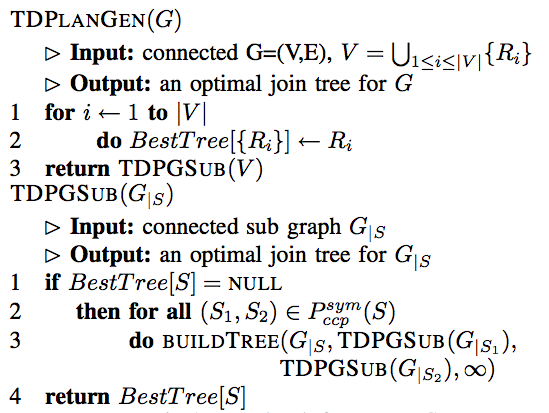
\includegraphics[width=9cm]{Figures/tdplangen.png}
\end{center}
\caption{Pseudocode for TDPLANGEN}
\label{fig:tdplangen}
\end{figure}

Depending on the choice of partitioning algorithm, the overall performance of \textsc{TDPlanGen} can vary by orders of magnitude. Since \textsc{TDPlanGen} is top-down  we can easily apply existing pruning techniques to prevent exploration of entire sub-trees. Later in section \ref{conservativePartitioning} we describe the \textsc{MinCutConservative} partitioning algorithm and how we can use it in transformational setting. 
\chapter{Effectiveness of Existing Rule Sets}
This chapter considers different rule sets used for join enumeration in transformation based query optimization using Volcano/Cascades framework and analyse them for:  
\begin{itemize}
	\item Completeness : Ability to generate the space of all cross-product free join orders starting from an initial plan without cross products.
	\item Efficiency : Number of duplicates generated in the process of exploring the space. The lower the better.
\end{itemize}

We start with a basic rule set consisting of commutativity and associativity called rule set RS-B0. RS-B0 consists of redundant rules  and this redundancy is addressed in rule set RS-B1. Pellenkoft et al.\cite{pellenkoft1997complexity} showed that using RS-B1 leads to the generation of an exponential number of duplicates. They presented a new rule set RS-B2 which uses a new rule 'Exchange' in conjunction with RS-B0 and some added constraints to generate all alternate bushy join trees without generating duplicates. However we show that RS-B2 achieves this by generating trees outside of search space and a restriction to remain in search space leads to incompleteness.

\begin{defn} 
A Join Graph is a pair H = (V,E) where V is the set of base relations $R_{1},...,R_{n}$ and E is a set of edges. An edge between $R_{i}$ and $R_{j}$ indicates presence of join predicate between them. 
\end{defn}

\begin{defn} 
A Query Tree Q is a bushy plan showing the way the relations will be joined together.
\end{defn}

\section{Rule set RS-B0}
The simplest set of rules used (to generate the bushy space) are :

\begin{itemize}
	\item Left Associativity \\ $A \bowtie (B \bowtie C) \rightarrow (A \bowtie B) \bowtie C$
	\item Right Associativity \\ ($A \bowtie B) \bowtie C \rightarrow A \bowtie (B \bowtie C)$
	\item Commutativity \\ $A \bowtie B \rightarrow B \bowtie A$
\end{itemize}

\subsection{Efficiency}
The set is redundant because we can drop Left (or Right) Associativity and still generate the same space. This redundancy is addressed in rule set RS-B1. The number of duplicates is atleast as many as RS-B1.

\subsection{Completeness}
We show later in section \ref{rsb1complete} that a subset of these rules is sufficient to enumerate the entire space. 

\section{Rule set RS-B1}
Rule set RS-B1 consists of subset of rules of RS-B0 namely :
\begin{itemize}
	\item Left Associativity \\ $A \bowtie (B \bowtie C) \rightarrow (A \bowtie B) \bowtie C$
	\item Commutativity \\ $A \bowtie B \rightarrow B \bowtie A$
\end{itemize}

\subsection{Efficiency}
Pellenkoft et al. \cite{pellenkoft1997complexity} have shown that RS-B1 leads to exponential number of duplicates. The number of duplicates generated during the construction of MEMO-structure encoding all bushy trees for a clique join graph on n relations is $4^{n}-3^{n+1}+2^{n+2}-n-2$.

\subsection{Completeness}
\label{rsb1complete}

We show that this minimal set is sufficient to enumerate the cross product free space assuming the query is fully connected. \\

\textbf{Problem Description} : Given a connected join graph J and query tree Q, show that using RS-B1 we can reach any other valid query tree Q' from Q while remaining in cross-product free space. \\

We assume that Q itself does not have any cross products ie: Q belongs to search space. Given the input join graph $J$ is completely connected we can number the nodes $1,2...n$ such that $(..(R_{1}\bowtie R_{2})...)\bowtie R{n}$ is a valid left-deep join tree. To prove the problem statement, we prove a stronger claim : \\

\textbf{Claim 1} : Any query tree can be transformed into left-deep join tree and left-deep join tree can be transformed into any query tree in the search space. Hence to go from query tree $Q_{1}$ to $Q_{2}$, there exists atleast one route ie: $Q_{1}$ to left-deep tree to $Q_{2}$\\

Let us break the process on conversion from one tree to another into steps. In step 1 we move $R_{n}$ to the top so that it is last relation to be joined and then work on remaining set of relations numbered $1,2,..,n-1$. Generalized in step $i$, we move relation $R_{n-i+1}$ to the top and recurse on remaining relations 1 ... n-i. The decent stops when $i=n-1$. This brings us to Claim 2. \\

\textbf{Claim 2}: Having a query tree with relations $R_{1},R_{2},...R_{k}$, it is possible to build tree $[R_{1}R_{2}..R_{k-1}] \bowtie R_{k}$ where $[R_{1}R_{2}..R_{k-1}]$ represents a smaller join tree with relations $R_{1},R_{2},..R_{k-1}$ \\

Now the goal is given an query graph, move the highest numbered relation to the top so that its the last relation to be joined. Let k be the highest numbered relation and 1 .. k-1 are the other relations in the graph. View the tree as in Figure \ref{fig:rsb1-proof} where $C_{1}, C_{2}, ... C_{m}$ are equivalence classes consisting of some number of relations. We say the height of the tree is m+1. By induction on tree height, we show that $R_{k}$ can be brought to top while remaining in cross-product free space. \\

\begin{figure}[here]
\begin{center}
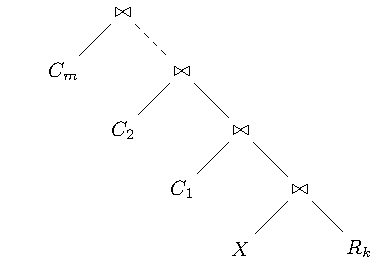
\includegraphics{Figures/rsb1-proof.pdf}
\end{center}
\caption{Reduced Query Tree}
\label{fig:rsb1-proof}
\end{figure}

Base Cases: When m = 0 , there is nothing to do, just repeat the procedure on X. When m = 1, X and $C_{1}$ should have a join predicate between them (because $R_{k}$ is the last relation to be join in left-deep tree). Applying left associativity we get required tree.\\

Induction on height m: Assume claim 2 holds for height $m <= j$. For height $m = j+1$, we know that since $R_{k}$ was the last relation to be joined in the left-deep tree, X can be joined with atleast one of the other C's say $C_{i}$. Pull $C_{i}$ down to X using a sequence of $C \rightarrow LA \rightarrow C$. Finally use Left Associativity to reduce height to j which is solvable. Hence Claim 2 proved, we can convert any tree into left-deep tree chosen earlier. \\

The last thing remaining to be shown is how we can go from left-deep tree to any other join tree. It is not difficult to see that this is equivalent to have the rules right associativity and commutativity and going from the join tree to left-deep tree. Right associativity can be done using a sequence of left associativity and commutativity : $RA \Rightarrow C \rightarrow C \rightarrow LA \rightarrow C$. We can use the same arguments as above to complete the proof.

\section{Rule set RS-B2}

Pellenkoft et al. \cite{pellenkoft1997complexity} presented a modified rule-set which generates the space of all bushy join trees with no duplicates. The rule set : 

\begin{itemize}
	\item $R_{1}$ : Commutativity \\ $A \bowtie_{0} B \rightarrow B \bowtie_{1} A$ \\
	Disable 	$R_{1}, R_{2}, R_{3}, R_{4}$ for application on new operator $\bowtie_{1}$
	\item $R_{2}$ : Left Associativity \\ $A \bowtie_{0} (B \bowtie_{1} C) \rightarrow (A \bowtie_{2} B) \bowtie_{3} C$ \\ 
	Disable 	$R_{2}, R_{3}, R_{4}$ for application  on new operator $\bowtie_{3}$	
	\item $R_{3}$ : Right Associativity \\ $(A \bowtie_{0} B) \bowtie_{1} C \rightarrow A \bowtie_{2} (B \bowtie_{3} C)$ \\
	Disable $R_{2}, R_{3}, R_{4}$ for application on new operator $\bowtie_{2}$	
	\item $R_{4}$ : Exchange \\ $(A \bowtie_{0} B) \bowtie_{1} (C \bowtie_{2} D) \rightarrow (A \bowtie_{3} C) \bowtie_{4} (B \bowtie_{5} D)$ \\
	Disable 	$R_{1}, R_{2}, R_{3}, R_{4}$ for application on new operator $\bowtie_{4}$
\end{itemize}

It is interesting to visualize the way exploration happens using RS-B2. Start at the topmost join operator, its left and right subtrees are completely explored. All the rules are applied at the top join operator and it gets locked. Now we explore all the newly generated join trees. In a way the locking happens one round from bottom to top, exchanges happen at the top(root) join operator and the root operator gets locked. Finally there is another round of locking happens this time from the top downwards. 

\subsection{Efficiency}
Pellenkoft et al. have showed that this scheme does not generate any duplicates and achieves the lower bound given by Ono and Lohman.


\subsection{Completeness}

\begin{figure}[ht]
\centering
\begin{subfigure}[b]{0.24\linewidth}
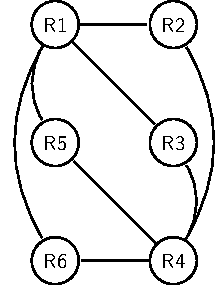
\includegraphics[width=2cm]{Figures/rsb2-predicates.pdf}
\caption{Join Graph J}
\label{fig:rsb2-counter}
\end{subfigure}
\begin{subfigure}[b]{0.35\linewidth}
	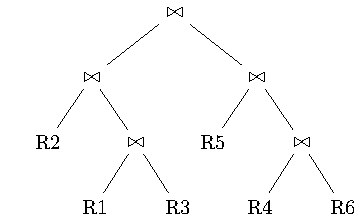
\includegraphics[width=3.5cm]{Figures/rsb2-counter.pdf}
\caption{Query Tree $Q$}
\label{fig:minipage1}
\end{subfigure}
\begin{subfigure}[b]{0.35\linewidth}
	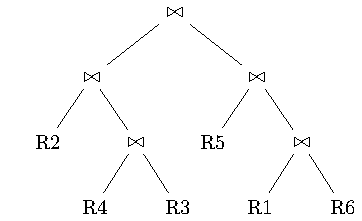
\includegraphics[width=3.5cm]{Figures/rsb2-counter2.pdf}
\caption{Query Tree $Q_{2}$}
\label{fig:minipage2}
\end{subfigure}
\end{figure}
RS-B2 cannot generate the space of all bushy trees without cross products. Given a set of relations to be joined with join graph $J$ (Figure \ref{fig:rsb2-counter}) and initial query tree $Q$ (Figure \ref{fig:minipage1}), observe that swapping R1 and R4 will lead to a valid query tree $Q_2$ (Figure \ref{fig:minipage2}) which does not have any cross product. Hence $Q_2$ belongs to search space. However going from $Q$ to $Q_2$ would require formation of sub-tree $R_2$,$R_3$ which will lead to cross product.
\chapter{Ruleset RS-B3}
In this chapter we address the drawbacks of RS-B1 and ineffectiveness of RS-B2 with our new rule-set RS-B3 which explores the space of cross product free query trees generating order of magnitude lesser duplicates. Section 5.1 describes the rule-set and the locking details. Section 5.2 proves the ability of rule-set to explore the entire space. Section 5.3 shows the effectiveness of the new rule-set in terms of number of duplicates generated. 
%Finally in Section 5.4 we show some experimental results.
  
\section{Rule-set RS-B3}
Given an initial Query Tree Q, for all join nodes enable only $R_{1}$ and $R_{2}$.

\begin{itemize}
	\item $R_{1}$: Commutativity \\ $A \bowtie_{0} B \rightarrow B \bowtie_{1} A$ \\
	Disable $R_{1}$,$R_{2}$ for application on new operator $\bowtie_{1}$
	\item $R_{2}$: Right Associativity \\ $(A \bowtie_{0} B) \bowtie_{1} C \rightarrow A \bowtie_{2} (B \bowtie_{3} C)$ \\
	Disable $R_{1}$,$R_{2}$ for application on new operator $\bowtie_{2}$. Enable $R_{3}$ for application on new operator $\bowtie_{2}$.		
	\item $R_{3}$: Left Associativity \\ $A \bowtie_{0} (B \bowtie_{1} C) \rightarrow (A \bowtie_{2} B) \bowtie_{3} C$ \\
	Enable $R_{1}$ for application on new operator $\bowtie_{3}$.
\end{itemize}

\section{Completeness}
This method of enumeration is not complete. There exist edge cases. Consider for example join graph as shown in figure \ref{fig:extreme}. Let the initial element be $[R_{1}R_{2}R_{3}R_{4}]\bowtie[R_{5}R_{6}R_{7}R_{8}]$ and final element $[R_{1}R_{2}R_{5}R_{6}]\bowtie[R_{3}R_{4}R_{7}R_{8}]$. In the current scheme, it is not possible to do this. Also note that no locking constrains while restricting the number of times group of relations move around the join to 2 can achieve this. However the ray of hope is that using a small perturbation ie: moving $R_{4}$ to right hand side and then starting the enumeration will work. \\

Note that the case that broke RS-B2 (see Figure \ref{rsb2-counter}) can actually be explored by using RS-B3. The sequence of moves would be $[R_{1}R_{3}]$ moves across the top join operator using right associativity, this new equivalence class is explored and $[R_{4}R_{3}]$ brought back to left side using left associativity. 

\begin{figure}[here]
\begin{center}
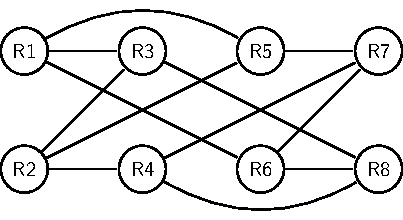
\includegraphics{Figures/extreme.pdf}
\end{center}
\caption{Extreme case for RS-B3}
\label{fig:extreme}
\end{figure}

\section{Number of Duplicates Generated}
\textbf{Claim 1}: The number of duplicates generated by \textbf{RS-B3} during the exploration of a class that combines k relations, on a completely connected graph is: $O(3^l2^r)$ \\
\textbf{Proof}: In a fully explored class that combines n relations the number of join operators is $A(n) = 2^n - 2$. Consider a class that combines $k$ relations. Using an initial element $[L]\bowtie[R]$ with $l$ the number of relations in $[L]$ and $k-l$ the number of relations in R, the transformation rules generate the following elements. Rule $R_{1}$ generates mirror image of original operator. Rule $R_{2}$ combines every element of $[L]$ with $[R]$. Note the previous step enables rule $R_{3}$. Now rule $R_{3}$ combines every element of this newly generated $[R']$ with the leftover of L. Counting the number of alternatives generates :
\begin{eqnarray*}
C &=& \sum\limits_{k=1}^{l-1} {l \choose k} A(k+r) \nonumber \\ 
 &=& \sum\limits_{k=1}^{l-1} {l \choose k} (2^{k+r} - 2) \nonumber \\
 &=& 2^r (3^l - 2^l - 1) - 2 (2^l - 2) \nonumber \\
\end{eqnarray*}

Application of rule $R_{3}$ enables commutativity which generates mirror images. To count the number of duplicates generated at this step add all the newly created operator and the initial operators and subtract $A(k)$ :
\begin{eqnarray*}
	D &=& 2 + 2*C - A(k) \nonumber \\
	  &=& 2 + 2^r (3^l - 2^l - 1) - 2 (2^l - 2) - (2^k - 2) \nonumber \\
	  &=& 3^l 2^r - 2^{k+1} - 2^r - 2^{l+1} +  8 \nonumber \\
\end{eqnarray*}
\chapter{Embedding Top-Down Join Enumerator}
\label{topdownint}
In this chapter we propose a new method of doing join enumeration in transformation-based optimizers based on ideas from memoization based join enumerators. DP-based and memoization-based enumeration algorithms\cite{fender2011new,fender2012effective,fender2013top} for join enumeration are more efficient in comparison to transformation-based ones in that they are able to enumerate the entire space without generating duplicates. 
In Section 6.1 we describe the algorithm, Section 6.2 describes the process for logical space generation and in  
Section 6.3 we describe a scheme for combining the two. 

\section{Conservative Partitioning}
\label{conservativePartitioning}
We describe in greater detail the conservative partitioning algorithm, denoted by \textsc{MinCutConservative} given by Pit Fender et al.\cite{fender2012effective}. The conservative partitioning algorithm is used in graph based join enumeration algorithm \textsc{TDMinCutConservative}. We try to use it here in a transformation based setting. \\

The algorithm emits all ccps for a connected vertex set $S \subseteq V$ where V is the vertex set of the query graph G=(V,E). The basic idea of conservative partitioning is to successively enhance a connected set C by members of its neighbourhood $N(C)$ at every recursive iteration. The process starts with a single vertex $t \in S$ through a redefinition of $N(\phi) = {t}$. This way, we ensure that at every instance of the algorithm's execution $C$ is connected. Since $S$ and $C \subset S$ are connected, for every possible complement $S \setminus C$ there must exist a join edge $(v1, v2)$, where $v1 \in C$ and $v2 \in (S \setminus C)$ holds. If at some point of enlarging $C$ its complement $S \setminus C$ in S is connected as well, the algorithm has found a ccp for S. \\

\begin{figure}[here]
\begin{center}
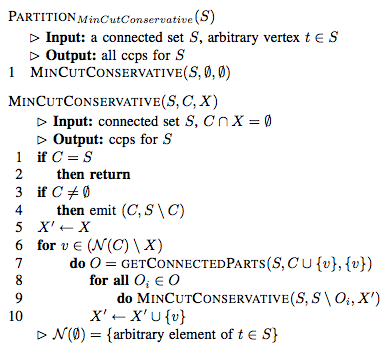
\includegraphics[width=9cm]{Figures/mincutconservative.png}
\end{center}
\caption{Pseudocode for \textsc{MinCutConservative}}
\label{fig:mincutconservative}
\end{figure}

\textsc{MinCutConservative} performs well even on when star queries are considered, where constructing every possible connected subset C of S produces an exponential overhead because most of the complements $S \setminus C$ are not connected and the partitions $(C, S \setminus C)$ computed this way are not valid ccps. Since the set C is expanded conservatively, this method remains effective. For pseudocode of the algorithm see Figure \ref{fig:mincutconservative}.

\section{Using Graph based enumeration}
We replace the existing join enumeration rules for commutativity and left associativity with a new  \textsc{N-ary Join} rule. The \textsc{N-ary Join} rule generates all ccps for the given set of n-relations. It is in essence a vanilla coated \textsc{MinCutConservative} algorithm.

\begin{defn}
A base equivalence class is defined as an equivalence class which is either a base relation or has atleast one  child logical operation node which is not a join operator.
\end{defn}

To run the \textsc{MinCutConservative} algorithm, we need the join graph induced by the base equivalence classes. For this we store two additional sets at each equivalence node:

\begin{itemize}
	\item \textsc{EqSet} : A set of all combinations of base equivalence classes being joined to generate this equivalence class. Along with this we need to store the ids of join operators of a feasible join ordering for these base equivalence class. This is used to infer the join graph.
	\item \textsc{HSet} : A set of hashes. For every set of base equivalence class that we enumerate, we generate a hash and store it in the parent equivalence class as a proof that this set has been enumerated. This is to prevent repeated enumeration of the same set of base equivalence classes.
\end{itemize}

Given with the above information, when \textsc{N-ary Join} rule is applied at a logical join operator $op$ get the \textsc{EqSet} of the left child and right child. For all combination of $S=S_{1} \cup S_{2}$ where $S_{1}\in \textsc{EqSet}_{L}$ and $S_{2}\in \textsc{EqSet}_{R}$, generate $hash(S)$ and check to ensure it has not been enumerated before. It it has not been enumerated, call \textsc{MinCutConservative}$(G_{|S})$. For every ccp generated add a new operation node to $child(parent(op))$. For every new equivalence class generated, insert it as a left-deep tree got by doing a depth-first traversal on the join graph (such a tree exists as the graph induced by these base equivalence classes is connected).

\chapter{Future Work}
Over the course of BTP, we have identified a number of promising areas related to query optimization in transformation-based query optimizers for future work :
\begin{itemize}
	\item \textbf{Memoization based Join Enumeration} : We plan to experiment with memoization-based join enumerator as a replacement for existing join enumeration rules (see Section \ref{topdownint}). The benefits and overheads need to be analysed.
	\item \textbf{Throw in more join operators} : We plan to analyse effect of adding in more operators like left outer join, full outer join, anti join, semi join and group joins into the bucket of join operators. Even with this extended family of join operators we aim at exploring the space of all valid plans without introducing cross products. 
	\item \textbf{Sampling the Search Space} : The search space grows exponentially with respect to number of relations. The idea is to generate a sample of the search space and from this sample give the optimal plan. Galindo-Legaria et al. \cite{galindo1995uniformly} presented a method for uniform random sample of all join orders. The problems we plan to tackle :
	\begin{itemize}
		\item Random sample of space of bushy join trees
		\item Extending to generating random sample of search space even in presence of other operators
	\end{itemize}
	\item \textbf{Prioritized Search Space Exploration} : Currently the search space is explored depth first. This approach is simple, however has inherent problem that we don't assign priority for traversal of children. Pruning depends on the order of exploration and hence it might be beneficial to assign 'priority' to each of the children and choose order based on this. Some ideas in \cite{fender2012effective}.	
	\item \textbf{Extending to Cascades and Columbia}: The Cascades optimizer generator overcomes many of the shortcomings of Volcano. We wish to check the applicability of things discussed in this report for use in Cascades style framework.	
\end{itemize}
\chapter{Conclusion}
In this report we presented :
\begin{itemize}
	\item An overview of query optimization process
	\item Literature survey of join enumeration techniques used
	\item Proofs of effectiveness/ineffectiveness of existing rule sets in exploring the space of all valid join trees without cross products
	\item New rule set RS-B3 for join enumeration
	\item New technique for complete enumeration without duplicates 
\end{itemize}
\pagenumbering{roman}
\printbibliography[heading=bibintoc]

\end{document}